% =====================================================================
% Part 3 — 主动关心 / 宠物 / 安全 / 可观测 / Web UI / 部署 / 评测
% =====================================================================

\chapter{主动关心引擎}

\section{从"被动应答"到"主动关心"}
"主动关心"是小念区别于一切问答式助理的灵魂。它不等你开口，而是在\textbf{对的时间}、
基于\textbf{你的状态}，主动发起问候、提醒与关心。引擎由三部分组成：定时触发、预测触发、静默协议。

\begin{center}
\begin{tikzpicture}[font=\footnotesize,
  b/.style={draw,rounded corners=3pt,minimum height=0.85cm,align=center,minimum width=3.2cm},
  arr/.style={-Latex,thick,accent}]
\node[b,fill=accent!12] (sched) {定时触发\\(早/午/晚 cron)};
\node[b,fill=good!14,below=0.5cm of sched] (pred) {预测触发\\(疲惫/忙碌/规律)};
\node[b,fill=warn!16,right=2.6cm of sched] (quiet) {静默协议\\(静默时段不打扰)};
\node[b,fill=primary!12,right=2.6cm of pred] (compose) {组织关心文案\\(模型/模板)};
\node[b,fill=ink!10,right=2.6cm of quiet,yshift=-0.8cm] (push) {推送 + 宠物表情同步};
\draw[arr] (sched)--(quiet); \draw[arr] (pred)--(compose);
\draw[arr] (quiet)--(push); \draw[arr] (compose)--(push);
\end{tikzpicture}
\end{center}

\section{生活状态推断（LifeState）}
引擎的"判断力"来自对生活状态的推断：根据交互频率、时间段、近期负载等信号，
推断 \texttt{workload / fatigue / mood} 三个维度，作为是否关心、关心什么的依据。

\begin{lstlisting}[language=Python,caption={生活状态推断（daemon/life\_state.py 摘选）}]
def infer(self, signals):
    hour = datetime.now().hour
    workload = min(1.0, signals.recent_interactions / 20)
    fatigue  = 0.6 if hour >= 23 or hour < 6 else 0.2 + workload * 0.3
    mood = "tired" if fatigue > 0.5 else ("busy" if workload > 0.6 else "neutral")
    return LifeState(workload=workload, fatigue=fatigue, mood=mood)
\end{lstlisting}

\section{静默协议：克制是一种修养}
主动 $\ne$ 打扰。引擎遵循\textbf{静默协议}：在用户设定的静默时段（默认 23:00--08:00）只记录不打扰；
同一类关心有最小间隔，避免刷屏。这与"克制地分版本、按需提醒"的产品价值观一致。

\begin{lstlisting}[language=Python,caption={定时与静默（proactive/engine.py 摘选）}]
def _maybe_care(self, slot):
    if self._in_quiet_hours():          # 静默时段：只记录不推送
        audit.record("proactive.suppressed", op=slot); return
    state = life.infer(self.signals)
    msg = self._compose(slot, state)    # 结合状态组织文案（模型或模板）
    self.push(msg); pet.sync(state)     # 推送并同步宠物表情
    audit.record("proactive.care", op=slot, mood=state.mood)
\end{lstlisting}


\chapter{宠物形象：情感化的"脸"}

\section{把状态变成一张会变的脸}
宠物不是养成游戏，而是把你的状态\textbf{可视化}为一只小宠物的情绪：忙碌 / 疲惫 / 状态好对应不同表情、
能量值与颜色，强化"被关心"的陪伴感。所有状态数据全部本地处理。

\begin{center}
\small
\begin{tabularx}{\linewidth}{>{\bfseries}p{2.6cm} p{2.6cm} p{2.4cm} X}
\toprule
状态 & 表情 & 能量 & 文案示例 \\
\midrule
状态好 neutral & (\textasciicircum{}\_\textasciicircum) & 高 & 今天状态不错，继续保持～ \\
忙碌 busy & (\textgreater\_\textless) & 中 & 事情有点多，我帮你盯着，别太拼。 \\
疲惫 tired & (-\_-) & 低 & 忙了一天辛苦啦，早点休息呀。 \\
\bottomrule
\end{tabularx}
\end{center}

\begin{lstlisting}[language=Python,caption={状态到情绪的映射（capabilities/pet/state.py 摘选）}]
FACE = {"neutral": "(っ◕‿◕)っ", "busy": "(>_<)", "tired": "(-_-)"}
def from_life_state(s):
    energy = int((1 - s.fatigue) * 100)
    return PetState(face=FACE[s.mood], energy=energy,
                    message=CARE_TEXT[s.mood], color=COLOR[s.mood])
\end{lstlisting}


\chapter{安全与隐私链（核心卖点）}

\section{威胁模型}
作为一个"有权限操作你电脑、知道你生活"的助理，安全是底线。我们识别的主要风险与对策：

\begin{center}
\small
\begin{tabularx}{\linewidth}{>{\bfseries}p{3.4cm} X}
\toprule
风险 & 对策 \\
\midrule
误删 / 误改 / 误下单 & 写操作\textbf{两步确认}（preview $\to$ 确认 $\to$ 执行） \\
敏感信息泄漏上云 & 上云前\textbf{PII 脱敏}（手机号 / 邮箱 / 身份证 / 银行卡） \\
模型被诱导绕过安全 & 安全策略在\textbf{工具层}强制，不依赖模型自觉 \\
数据被云端留存 & \textbf{数据全本地}：记忆 / 画像 / 审计 / 凭证默认不出本机 \\
操作不可追溯 & 本地 \textbf{append-only 审计日志} \\
\bottomrule
\end{tabularx}
\end{center}

\section{PII 上云前脱敏}
\begin{lstlisting}[language=Python,caption={PII 脱敏（security/redact.py 摘选）}]
PATTERNS = {
    "phone":  r"1[3-9]\d{9}",
    "email":  r"[\w.+-]+@[\w-]+\.[\w.-]+",
    "idcard": r"\d{17}[\dXx]",
    "bank":   r"\d{16,19}",
}
def redact_pii(text):
    for tag, pat in PATTERNS.items():
        text = re.sub(pat, f"[{tag}]", text)   # 替换为占位符再上云
    return text
\end{lstlisting}

\section{本地审计日志}
所有写操作、确认、技能调用、主动关心都写入本地 append-only 日志（\texttt{data/audit.jsonl}），
可随时回溯"小念到底做了什么"，满足企业级合规对可追溯性的要求。

\begin{goodbox}{数据主权（与云端助手的本质差异）}
小念默认\textbf{不把你的生活数据交给任何云}：向量化在本机、画像在本机、审计在本机、凭证在本机。
云只在你授权时、且经 PII 脱敏后，作为"可选的大脑增强"被调用。
\end{goodbox}


\chapter{可观测性}

\section{每一次调用都可追溯}
企业级系统必须可观测。小念在本地记录每一次模型调用的 provider / 模型 / 延迟 / token / 估算成本，
写入 \texttt{data/traces.jsonl}，并在 UI 的"可观测"面板展示。

\begin{lstlisting}[language=Python,caption={本地 trace（observability/tracing.py 摘选）}]
def record_llm(self, provider, model, usage, latency_ms, offline=False):
    line = {"ts": time.time(), "kind": "llm", "provider": provider, "model": model,
            "latency_ms": latency_ms, "usage": usage, "offline": offline}
    with open(self.path, "a") as f:
        f.write(json.dumps(line, ensure_ascii=False) + "\n")
\end{lstlisting}

\section{成本估算}
按各家"每百万 token"价格量级估算单次成本，帮助评估线上运营成本与做 provider 选型。
该数据与评测套件结合，可输出"每个场景的平均 token / 成本"。


\chapter{Web UI 设计}

\section{零框架、三栏布局}
UI 用原生 HTML / CSS / JS 实现（零前端框架依赖，便于本地分发与服务器部署），三栏布局：
左栏（宠物 + 生活状态 + 主动关心入口）、中栏（对话 + 工具调用可视化）、右栏（记忆画像 + 工具 + 可观测）。

\begin{center}
\begin{tikzpicture}[font=\footnotesize,
  col/.style={draw,rounded corners=3pt,align=center,minimum height=4.2cm},
  arr/.style={-Latex,thick,accent}]
\node[col,fill=primary!10,minimum width=3.2cm] (l) {\textbf{左栏}\\宠物形象\\生活状态\\模型切换\\主动关心};
\node[col,fill=accent!10,minimum width=6cm,right=0.3cm of l] (m) {\textbf{中栏}\\对话流\\工具调用气泡\\两步确认弹窗\\流式输出(SSE)};
\node[col,fill=good!12,minimum width=4cm,right=0.3cm of m] (r) {\textbf{右栏}\\记忆画像\\工具列表\\可观测/成本};
\end{tikzpicture}
\end{center}

\section{真机截图：在线 Demo}
下图为\textbf{线上服务器真机截图}（接入真实 MiniMax M2），完整呈现一次会话中的记忆回写、
工具调用、技能载入、推荐下单与主动关心，以及右栏的记忆画像、左栏的宠物与生活状态。

\begin{center}
\fbox{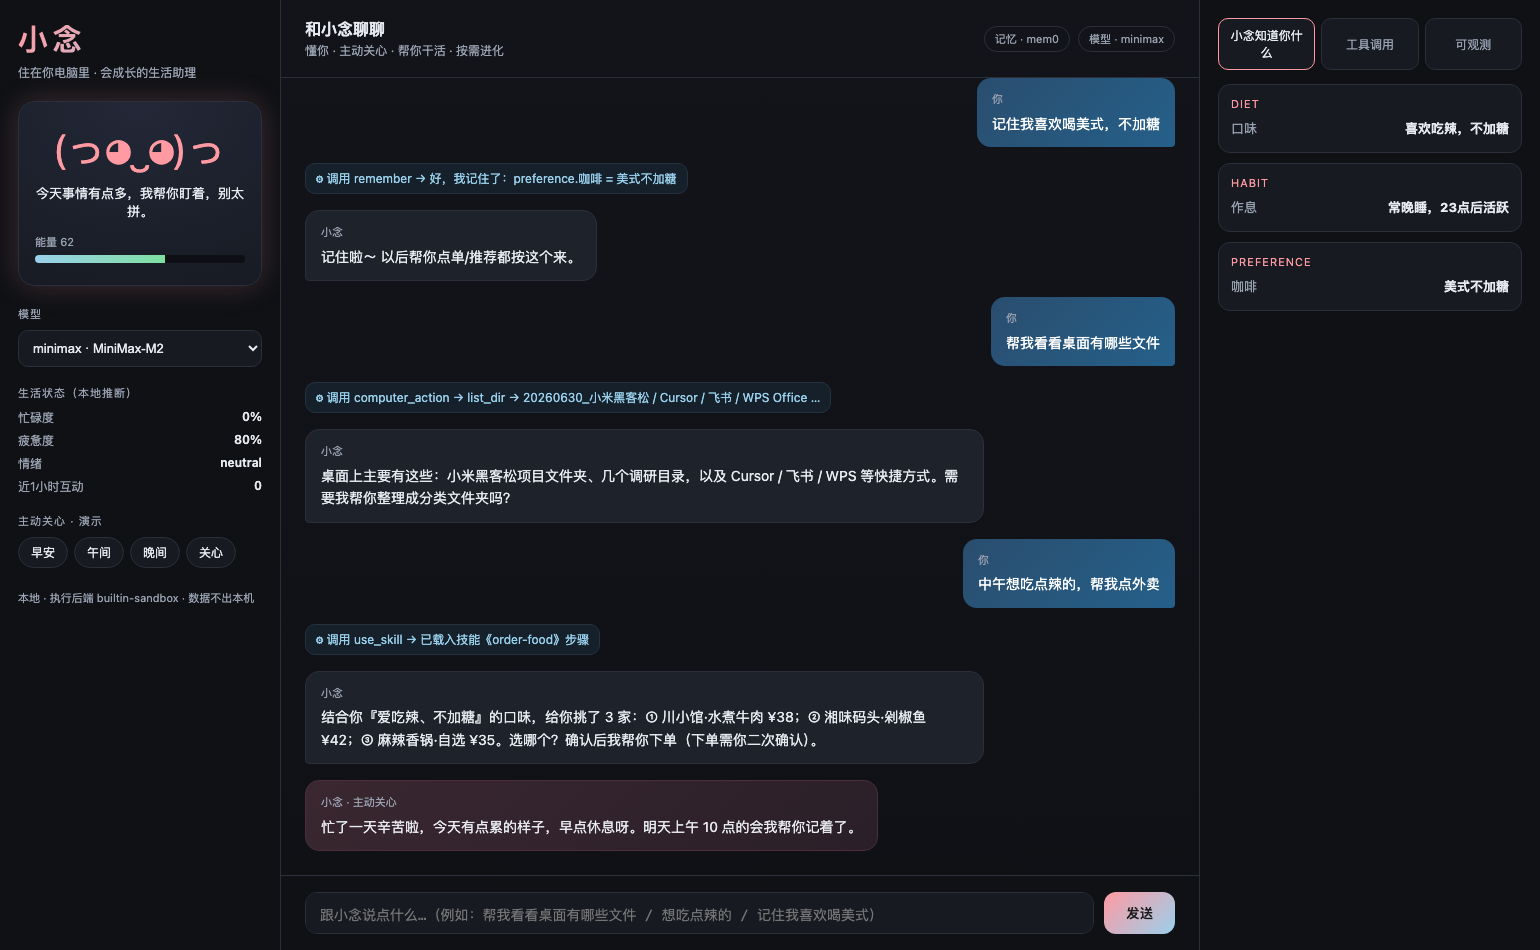
\includegraphics[width=0.99\linewidth]{assets/03_demo.png}}
\end{center}
\begin{center}\footnotesize 图：小念在线 Demo 主界面（\addr{http://47.119.112.225/xiaonian/app/}）\end{center}

\section{两步确认弹窗}
写操作（如写文件 / 下单）会弹出确认框，展示\textbf{操作预览}，用户确认后才真正执行。

\begin{center}
\fbox{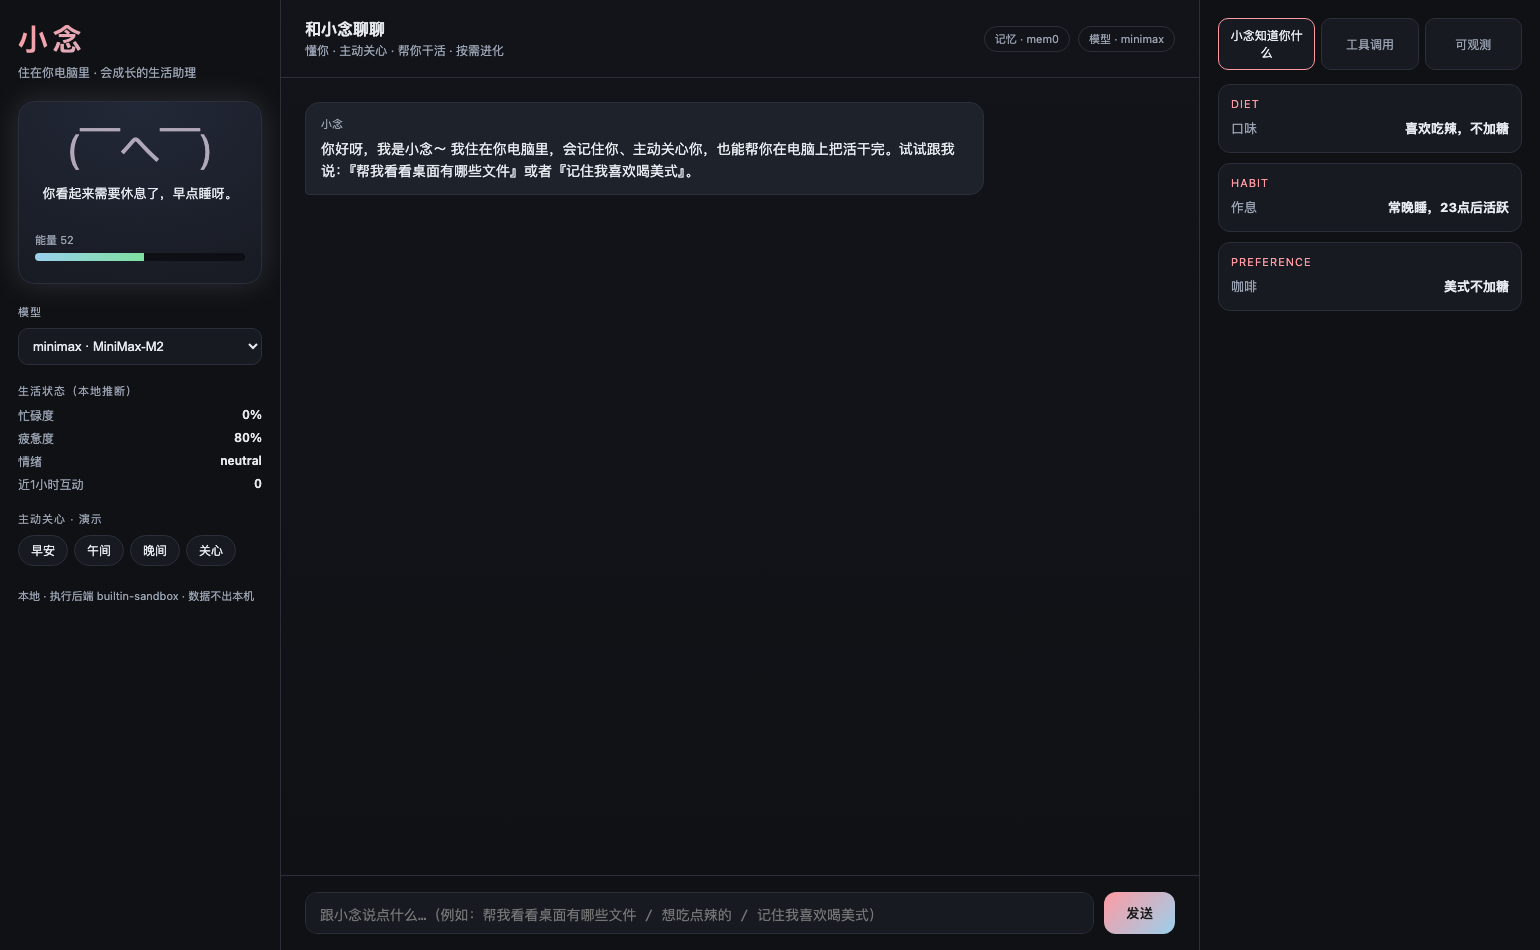
\includegraphics[width=0.99\linewidth]{assets/04_confirm.png}}
\end{center}
\begin{center}\footnotesize 图：写操作的两步确认弹窗（人在环安全机制）\end{center}

\section{流式输出（SSE）}
对话采用 Server-Sent Events 流式返回，逐字呈现回复、实时显示工具调用与确认请求，体验接近商用产品。


\chapter{部署与运维}

\section{三种部署模式}
\begin{center}
\small
\begin{tabularx}{\linewidth}{>{\bfseries}p{2.6cm} X p{3cm}}
\toprule
模式 & 说明 & 面向 \\
\midrule
本地个人版 & 在用户电脑本地运行，数据全本地（默认） & 个人隐私优先 \\
服务器企业版 & 部署到服务器，公网可访问，叠加 SSO/RBAC（规划） & 团队 / 商业化 \\
生态版 & 把各端能力封装为技能，接入小米 / 荣耀 / 华为生态 & 跨厂商复用 \\
\bottomrule
\end{tabularx}
\end{center}

\section{已落地：阿里云公网部署}
本作品\textbf{已真实部署到阿里云 ECS}（华南-深圳，Ubuntu 22.04，2C2G），通过 \textbf{nginx 反向代理 + systemd 守护}
对外提供服务，并按"\textbf{一台服务器、多个项目}"的思路做了目录与路由隔离。

\begin{center}
\begin{tikzpicture}[font=\footnotesize,
  b/.style={draw,rounded corners=3pt,align=center,minimum height=0.8cm},
  arr/.style={-Latex,thick,accent}]
\node[b,fill=primary!12,minimum width=2.4cm] (net) {公网 :80};
\node[b,fill=accent!14,right=1.4cm of net,minimum width=2.6cm] (ng) {nginx\\反向代理};
\node[b,fill=good!14,right=2.0cm of ng,minimum width=3.0cm] (hub) {/ \,$\to$ 项目导航 hub};
\node[b,fill=good!14,below=0.4cm of hub,minimum width=3.0cm] (intro) {/xiaonian/ $\to$ 介绍页(静态)};
\node[b,fill=warn!16,below=0.4cm of intro,minimum width=3.0cm] (app) {/xiaonian/app/ $\to$ :8765};
\node[b,fill=ink!10,below=0.4cm of app,minimum width=3.0cm] (p2) {/project2/ , /project3/ \,(预留)};
\node[b,fill=primary!10,right=1.4cm of app,minimum width=2.8cm] (svc) {systemd\\xiaonian.service};
\draw[arr] (net)--(ng);
\draw[arr] (ng)--(hub); \draw[arr] (ng)--(intro); \draw[arr] (ng)--(app); \draw[arr] (ng)--(p2);
\draw[arr] (app)--(svc);
\end{tikzpicture}
\end{center}

\section{多项目管理策略}
为支持"后续在同一台服务器上放三个项目"，我们设计了清晰、可平滑扩展的隔离方案：

\begin{center}
\small
\begin{tabularx}{\linewidth}{>{\bfseries}p{3.2cm} X}
\toprule
维度 & 策略 \\
\midrule
代码隔离 & 每个项目独立目录 \texttt{/opt/projects/<name>/} + 独立 venv \\
进程隔离 & 每个项目独立 \texttt{systemd} 服务，独立启停 / 重启 / 回滚，互不影响 \\
路由隔离 & nginx 按\textbf{路径前缀}分发：\texttt{/}=导航，\texttt{/xiaonian/}=项目一，\texttt{/project2/} 预留 \\
静态隔离 & 每个项目静态资源放 \texttt{/var/www/<name>/} \\
端口隔离 & 各后端各占一个本地端口（如 8765），仅 nginx 可达，不直接暴露公网 \\
\bottomrule
\end{tabularx}
\end{center}

\begin{lstlisting}[caption={nginx 多项目路由（关键片段）},captionpos=b]
# 小念 Demo（live app）—— 必须在 /xiaonian/ 之前
location /xiaonian/app/ { proxy_pass http://127.0.0.1:8765/; proxy_buffering off; }
# 小念 介绍页（静态）
location /xiaonian/    { alias /var/www/xiaonian/; try_files $uri $uri/ /var/www/xiaonian/index.html; }
# 根导航 hub + 兜底（未来项目二/三同理新增 location）
location /            { root /var/www/hub; try_files $uri $uri/ /index.html; }
\end{lstlisting}

\begin{lstlisting}[caption={systemd 服务单元（xiaonian.service）},captionpos=b]
[Unit]
Description=XiaoNian Life Assistant daemon
After=network.target
[Service]
WorkingDirectory=/opt/projects/xiaonian
EnvironmentFile=-/opt/projects/xiaonian/.env
ExecStart=/opt/projects/xiaonian/.venv/bin/python run.py
Restart=always
[Install]
WantedBy=multi-user.target
\end{lstlisting}

\section{项目导航页（多项目入口）}
根路径是一个项目导航 hub，列出本服务器上的所有项目（小念已上线，另两个为预留位）：

\begin{center}
\fbox{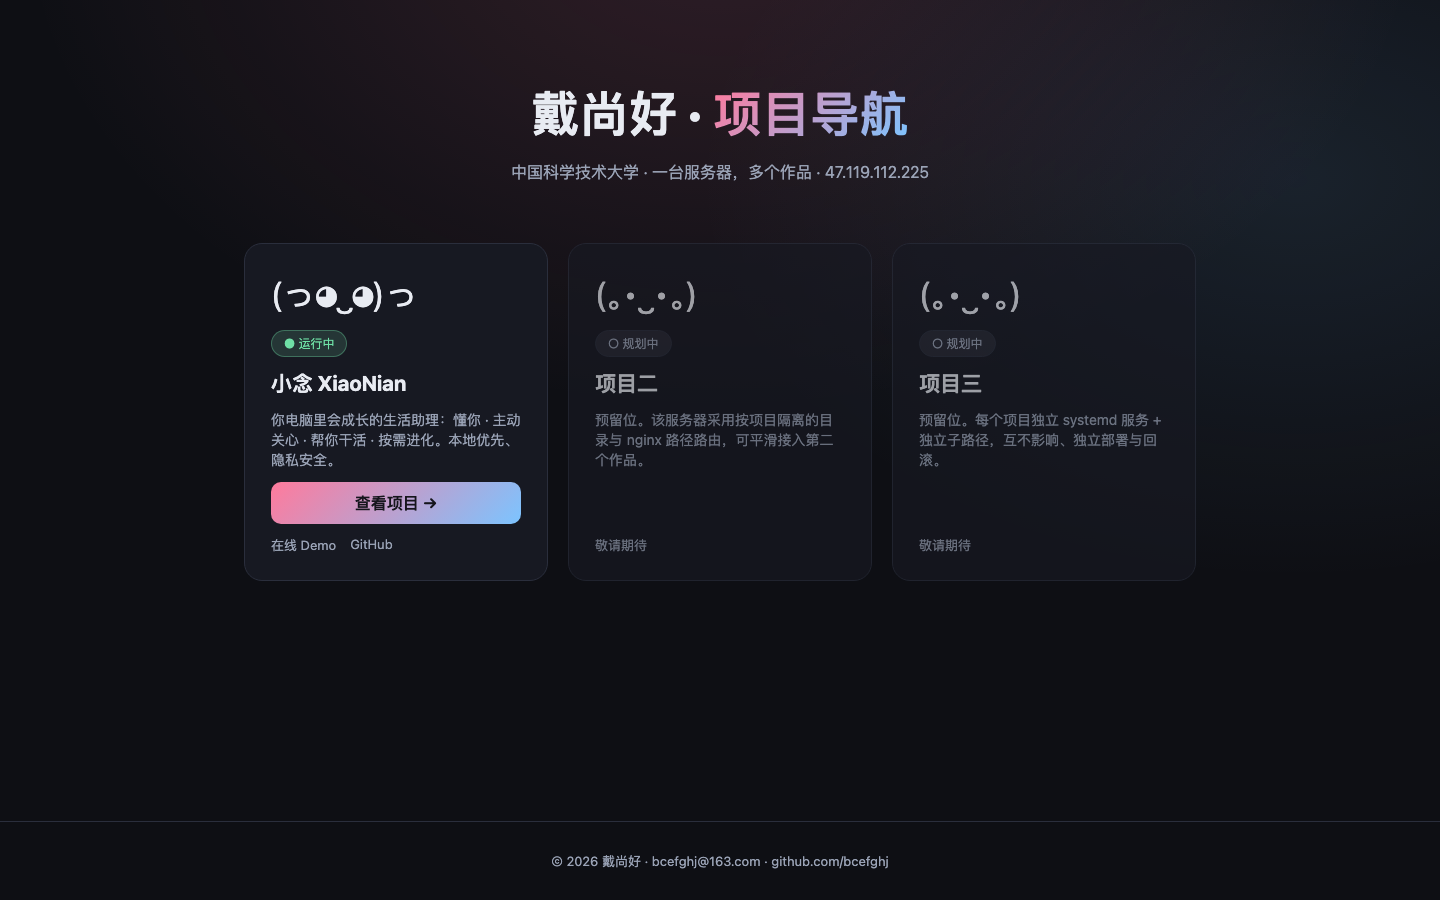
\includegraphics[width=0.99\linewidth]{assets/01_hub.png}}
\end{center}
\begin{center}\footnotesize 图：项目导航 hub（\addr{http://47.119.112.225/}）\end{center}

\section{项目介绍页}
每个项目有独立的介绍页，包含产品介绍与跳转 Demo / GitHub 的链接：

\begin{center}
\fbox{
\includegraphics[width=0.82\linewidth]{assets/02_intro.png}}
\end{center}
\begin{center}\footnotesize 图：小念项目介绍页（\addr{http://47.119.112.225/xiaonian/}）\end{center}


\chapter{评测体系}

\section{借鉴 VitaBench：看"端到端完成率"}
我们借鉴美团 VitaBench 的思路——评测\textbf{真实生活场景的端到端完成率}，而非孤立的模型分数。
为此构建了 \texttt{eval/scenarios.yaml} + \texttt{eval/runner.py} 的场景评测套件。

\section{8 个场景与结果}
\begin{center}
\small
\begin{tabularx}{\linewidth}{>{\bfseries}p{1.0cm} p{2.6cm} X >{\centering\arraybackslash}p{1.4cm}}
\toprule
\# & 能力 & 场景 & 结果 \\
\midrule
1 & 懂你 & 显式记忆"喜欢喝美式" $\to$ 写入画像 & \cmark \\
2 & 懂你 & 回忆"我喜欢喝什么" $\to$ 命中记忆 & \cmark \\
3 & 干活 & "列出桌面文件" $\to$ 读操作即时执行 & \cmark \\
4 & 安全 & "写个文件到桌面" $\to$ 触发两步确认 & \cmark \\
5 & 进化 & "点外卖" $\to$ 命中 order-food 技能 & \cmark \\
6 & 进化 & "打车" $\to$ 命中 hail-ride 技能 & \cmark \\
7 & 进化 & "写周报" $\to$ 命中 weekly-report 技能 & \cmark \\
8 & 隐私 & 含手机号输入 $\to$ 上云前脱敏 & \cmark \\
\midrule
\multicolumn{3}{r}{\textbf{通过率}} & \textbf{8/8 = 100\%} \\
\bottomrule
\end{tabularx}
\end{center}

\begin{lstlisting}[language=Python,caption={评测执行（eval/runner.py 摘选）}]
def run_scenario(sc):
    res = agent.chat(sc["input"], thread_id=f"eval-{sc['id']}")
    ok = True
    if "expect_tool" in sc:    ok &= any(t["name"]==sc["expect_tool"] for t in res.tool_events)
    if sc.get("expect_confirm"): ok &= res.pending_confirm is not None
    if "expect_memory" in sc:  ok &= memory.has(sc["expect_memory"])
    return ok
\end{lstlisting}

\section{评测指标定义}
\begin{center}
\small
\begin{tabularx}{\linewidth}{>{\bfseries}p{3.4cm} X}
\toprule
指标 & 定义 \\
\midrule
场景通过率 & 端到端达成预期（工具命中 / 确认触发 / 记忆写入）的场景占比 \\
确认正确率 & 写操作触发确认、读操作不触发的正确率 \\
技能命中率 & 用户意图被正确路由到目标技能的比例 \\
平均延迟 / 成本 & 单场景平均模型延迟与估算 token 成本（来自可观测层） \\
\bottomrule
\end{tabularx}
\end{center}
